%%%%%%%%%%%%%%%%%%%%%%%%%%%%%%%%%%%%%%%%%%%%%%%%%%%%%%%%%%%%%%%%%%%%%%%
% 
%%%%%%%%%%%%%%%%%%%%%%%%%%%%%%%%%%%%%%%%%%%%%%%%%%%%%%%%%%%%%%%%%%%%%%%

\chapter{\babEmpat}

%%%%%%%%%%%%%%%%%%%%%%%%%%%%%%%%%%%%%%%%%%%%%%%%%%%%%%%%%%%%%%%%%%%%%%%
% 
%%%%%%%%%%%%%%%%%%%%%%%%%%%%%%%%%%%%%%%%%%%%%%%%%%%%%%%%%%%%%%%%%%%%%%%

\section{Pengujian}
Setelah desain selesai di rancang, kemudian dilakukan pengujian untuk mengetahui apakah desain yang telah dirancang dapat bekerja dengan baik serta mengetahui bagaimana performasi alat yang di rancang.

\subsection{Sekenario Pengujian}
Untuk pengujian yang dilakukan adalah pengujian funsional algoritma (behavioral) serta pengujian performansi waktu operasi dan daya yang dibutuhkan alat yang telah dirancang.

Pada pengujian fungsional dilakukan pengujian mengguankan simulasi diagram waktu. Pada diagram waktu dapat dilihat proses input output satu demi satu dalam satuan waktu tertentu. Pengujian satu persatu dilakukan untuk mengetahui secara detail fungsional IC yang telah dirancang.

Apabila uji fungsional tidak ditemukan anomali, maka dilanjutkan pengujian selanjutnya yaitu pengujian daya serta performansi. Hal ini untuk mengetahui apakah terjadi perubahan yang signifikan pada perangkat yang diberi perlindungan dengan yang tidak diberi perlindungan

\subsection{Hasil Pengujian}
Berikut ini adalah hasil pengujian fungsional dari perangkat yang telah dilindungi. pengujian yang pertama adalah pengujian fungsional  modul inti yaitu modul ALU.

\begin{table}[H]
	\centering
	\caption{Data Mentah}
	\label{tab:rawdata}%
	\begin{tabular}{|c|c|c|c|c|c|c|c|c|c|c|c|c|c|c|c|c|c|}
		\hline
		\rowcolor[rgb]{ .949,  .949,  .949} \multicolumn{18}{|c|}{REG} \bigstrut\\
		\hline
		\rowcolor[rgb]{ .949,  .949,  .949} \multicolumn{1}{|p{2.145em}|}{CLK} & \multicolumn{8}{c|}{A}                                        &       & \multicolumn{8}{c|}{Z} \bigstrut\\
		\hline
		0     & 0     & 0     & 0     & 0     & 0     & 1     & 1     & 1     & \multirow{19}[38]{*}{} & 0     & 0     & 0     & 0     & 0     & 0     & 0     & 0 \bigstrut\\
		\cline{1-9}\cline{11-18}    1     & 0     & 0     & 0     & 0     & 0     & 1     & 0     & 1     &       & 0     & 1     & 0     & 0     & 0     & 0     & 0     & 0 \bigstrut\\
		\cline{1-9}\cline{11-18}    2     & 0     & 0     & 0     & 0     & 0     & 1     & 1     & 0     &       & 1     & 0     & 0     & 0     & 0     & 0     & 0     & 0 \bigstrut\\
		\cline{1-9}\cline{11-18}    3     & 0     & 0     & 0     & 0     & 0     & 0     & 1     & 0     &       & 1     & 1     & 0     & 0     & 1     & 0     & 1     & 0 \bigstrut\\
		\cline{1-9}\cline{11-18}    4     & 0     & 0     & 0     & 0     & 0     & 0     & 1     & 1     &       & 0     & 0     & 0     & 0     & 1     & 0     & 1     & 0 \bigstrut\\
		\cline{1-9}\cline{11-18}    5     & 0     & 0     & 0     & 0     & 0     & 1     & 0     & 0     &       & 0     & 1     & 0     & 0     & 1     & 0     & 1     & 0 \bigstrut\\
		\cline{1-9}\cline{11-18}    6     & 0     & 0     & 0     & 0     & 0     & 0     & 1     & 0     &       & 1     & 0     & 0     & 0     & 1     & 0     & 1     & 0 \bigstrut\\
		\cline{1-9}\cline{11-18}    7     & 0     & 0     & 0     & 0     & 0     & 0     & 0     & 0     &       & 1     & 1     & 0     & 1     & 0     & 0     & 0     & 0 \bigstrut\\
		\cline{1-9}\cline{11-18}    8     & 0     & 0     & 0     & 0     & 0     & 1     & 1     & 1     &       & 0     & 0     & 0     & 1     & 0     & 0     & 0     & 0 \bigstrut\\
		\cline{1-9}\cline{11-18}    9     & 0     & 0     & 0     & 0     & 0     & 1     & 0     & 0     &       & 0     & 1     & 0     & 1     & 0     & 0     & 0     & 0 \bigstrut\\
		\cline{1-9}\cline{11-18}    10    & 0     & 0     & 0     & 0     & 0     & 0     & 1     & 0     &       & 1     & 0     & 0     & 1     & 0     & 0     & 0     & 0 \bigstrut\\
		\cline{1-9}\cline{11-18}    11    & 0     & 0     & 0     & 0     & 0     & 0     & 0     & 1     &       & 1     & 1     & 0     & 1     & 1     & 0     & 0     & 1 \bigstrut\\
		\cline{1-9}\cline{11-18}    12    & 0     & 0     & 0     & 0     & 0     & 1     & 0     & 1     &       & 0     & 0     & 0     & 1     & 1     & 0     & 0     & 1 \bigstrut\\
		\cline{1-9}\cline{11-18}    13    & 0     & 0     & 0     & 0     & 0     & 0     & 1     & 1     &       & 0     & 1     & 0     & 1     & 1     & 0     & 0     & 1 \bigstrut\\
		\cline{1-9}\cline{11-18}    14    & 0     & 0     & 0     & 0     & 0     & 0     & 1     & 1     &       & 1     & 0     & 0     & 1     & 1     & 0     & 0     & 1 \bigstrut\\
		\cline{1-9}\cline{11-18}    15    & 0     & 0     & 0     & 0     & 0     & 1     & 0     & 0     &       & 1     & 1     & 1     & 0     & 0     & 1     & 0     & 0 \bigstrut\\
		\cline{1-9}\cline{11-18}    16    & 0     & 0     & 0     & 0     & 0     & 0     & 1     & 0     &       & 0     & 0     & 1     & 0     & 0     & 1     & 0     & 0 \bigstrut\\
		\cline{1-9}\cline{11-18}    17    & 0     & 0     & 0     & 0     & 0     & 1     & 1     & 1     &       & 0     & 1     & 1     & 0     & 0     & 1     & 0     & 0 \bigstrut\\
		\cline{1-9}\cline{11-18}    18    & 0     & 0     & 0     & 0     & 0     & 0     & 1     & 1     &       & 1     & 0     & 1     & 0     & 0     & 1     & 0     & 0 \bigstrut\\
		\hline
	\end{tabular}%
\end{table}%

Data mentah (raw) di atas didapat dari hasil timing diagram (lampiran). Untuk mengetahui hasil kebenaran dilakukan truth prove pada data raw.

\begin{table}[H]
	\centering
	\caption{Analisis Data Mentah}
	\label{tab:translasi}%
	\begin{tabular}{|c|c|c|c|c|c|c|c|c|c|c|c|c|}
		\hline
		\rowcolor[rgb]{ .949,  .949,  .949} \multicolumn{2}{|c|}{IO} & \multicolumn{8}{c|}{bit}                                      & \multicolumn{3}{c|}{STEP} \bigstrut\\
		\hline
		\rowcolor[rgb]{ .949,  .949,  .949} in    & out   & 7     & 6     & 5     & 4     & 3     & 2     & 1     & 0     & HCUT  & MCUT  & \multicolumn{1}{l|}{CHECK} \bigstrut\\
		\hline
		7     & 0     & 128   & 64    & 32    & 16    & 8     & 4     & 2     & 1     & 0     & 0     & - \bigstrut\\
		\hline
		5     & 64    & 128   & 64    & 32    & 16    & 8     & 4     & 2     & 1     & 0     & 0     & - \bigstrut\\
		\hline
		6     & 128   & 128   & 64    & 32    & 16    & 8     & 4     & 2     & 1     & 0     & 0     & - \bigstrut\\
		\hline
		2     & 202   & 128   & 64    & 32    & 16    & 8     & 4     & 2     & 1     & 10    & 2     & OK \bigstrut\\
		\hline
		3     & 10    & 128   & 64    & 32    & 16    & 8     & 4     & 2     & 1     & 0     & 0     & - \bigstrut\\
		\hline
		4     & 74    & 128   & 64    & 32    & 16    & 8     & 4     & 2     & 1     & 0     & 0     & - \bigstrut\\
		\hline
		2     & 138   & 128   & 64    & 32    & 16    & 8     & 4     & 2     & 1     & 0     & 0     & - \bigstrut\\
		\hline
		0     & 208   & 128   & 64    & 32    & 16    & 8     & 4     & 2     & 1     & 16    & 0     & OK \bigstrut\\
		\hline
		7     & 16    & 128   & 64    & 32    & 16    & 8     & 4     & 2     & 1     & 0     & 0     & - \bigstrut\\
		\hline
		4     & 80    & 128   & 64    & 32    & 16    & 8     & 4     & 2     & 1     & 0     & 0     & - \bigstrut\\
		\hline
		2     & 144   & 128   & 64    & 32    & 16    & 8     & 4     & 2     & 1     & 0     & 0     & - \bigstrut\\
		\hline
		1     & 217   & 128   & 64    & 32    & 16    & 8     & 4     & 2     & 1     & 25    & 1     & OK \bigstrut\\
		\hline
		5     & 25    & 128   & 64    & 32    & 16    & 8     & 4     & 2     & 1     & 0     & 0     & - \bigstrut\\
		\hline
		3     & 89    & 128   & 64    & 32    & 16    & 8     & 4     & 2     & 1     & 0     & 0     & - \bigstrut\\
		\hline
		3     & 153   & 128   & 64    & 32    & 16    & 8     & 4     & 2     & 1     & 0     & 0     & - \bigstrut\\
		\hline
		4     & 228   & 128   & 64    & 32    & 16    & 8     & 4     & 2     & 1     & 36    & 4     & OK \bigstrut\\
		\hline
		2     & 36    & 128   & 64    & 32    & 16    & 8     & 4     & 2     & 1     & 0     & 0     & - \bigstrut\\
		\hline
		7     & 100   & 128   & 64    & 32    & 16    & 8     & 4     & 2     & 1     & 0     & 0     & - \bigstrut\\
		\hline
		3     & 164   & 128   & 64    & 32    & 16    & 8     & 4     & 2     & 1     & 0     & 0     & - \bigstrut\\
		\hline
	\end{tabular}%
\end{table}%

Dari hasil pengujian di atas didapat bahwa fungsional dari masing masing modul yang telah digabung tidak saling bentrok satu sama lain dan dapat bekerja dengan semestinya.

Dengan hasil pengujian fungsional yang tidak terdapat anomali maka dapat dilanjutkan analisis daya dari modul sebelum diberi perlindungan dengan modul yang telah diberi perlindungan.

%%%%%%%%%%%%%%%%%%%%%%%%%%%%%%%%%%%%%%%%%%%%%%%%%%%%%%%%%%%%%%%%%%%%%%%
% 
%%%%%%%%%%%%%%%%%%%%%%%%%%%%%%%%%%%%%%%%%%%%%%%%%%%%%%%%%%%%%%%%%%%%%%%

\section{Analisis}
Pertama analisis performansi perangkat sebelum dilindungi, kemudian lindungi alat dengan rangkaian pelindung dan analisis performansinya dan bandingkan hasil analisis sebelum dengan hasil analisis sesudah dilindungi. berikut rekap data hasil analisis sebelum dan sesudah diberi rangkaian pelindung. Berikut merupakan soft-estimasi kecepatan clock pada FPGA arsitektur XILINX.

\begin{table}[H]
	\centering
	\caption{FPGA Speed Analysis}
	\label{tab:speed}%
	\begin{tabular}{|l|c|c|}
		\hline
		\rowcolor[rgb]{ .906,  .902,  .902} \multicolumn{1}{|c|}{Unprotected} & Minimum & Maximum \bigstrut\\
		\hline
		Period & 2.692ns & 371.471MHz (freq) \bigstrut\\
		\hline
		Input arrival time before clock & 10.075ns & - \bigstrut\\
		\hline
		Output required time after clock & -     & 5.558ns \bigstrut\\
		\hline
		\rowcolor[rgb]{ .906,  .902,  .902} \multicolumn{1}{|c|}{Protected} & Minimum & Maximum \bigstrut\\
		\hline
		Period & 4.023ns & 248.571MHz (freq) \bigstrut\\
		\hline
		Input arrival time before clock & 8.667ns & - \bigstrut\\
		\hline
		Output required time after clock & -     & 6.962ns \bigstrut\\
		\hline
	\end{tabular}%
\end{table}%

Dari hasil analisis terjadi penurunan kecepatan maksimum proses pada FPGA dari 371.471 Mhz menjadi 248.571 Mhz atau sekitar 33\%. Pada hasil soft-simulasi ini mengindikasikan bakal terjadi penurunan speed pada modul yang sedang dikembangkan.

\begin{table}[H]
	\centering
	\caption{On-Chip Power Summary}
	\label{tab:power}%
	\begin{tabular}{|l|c|}
		\hline
		\rowcolor[rgb]{ .906,  .902,  .902} \multicolumn{1}{|c|}{Unprotected} & Power (mW) \bigstrut\\
		\hline
		Clock & 1.12 \bigstrut\\
		\hline
		Static Power & 10.42 \bigstrut\\
		\hline
		Total & 11.54 \bigstrut\\
		\hline
		\rowcolor[rgb]{ .906,  .902,  .902} \multicolumn{1}{|c|}{Protected} & Power (mW) \bigstrut\\
		\hline
		Clock & 1.37 \bigstrut\\
		\hline
		Static Power & 10.42 \bigstrut\\
		\hline
		Total & 11.79 \bigstrut\\
		\hline
	\end{tabular}%
\end{table}%

\begin{figure}
	\centering
	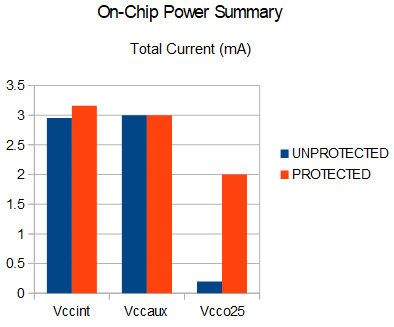
\includegraphics[width=0.5\textwidth]
	{pics/total_current.png}
	\caption{totalcurrent}
	\label{total_current}
\end{figure}

\begin{figure}
	\centering
	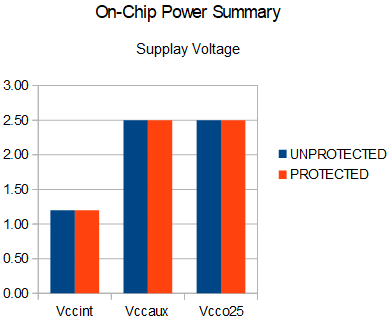
\includegraphics[width=0.5\textwidth]
	{pics/suplay_voltage.png}
	\caption{suplayvoltage}
	\label{suplay_voltage}
\end{figure}

\begin{figure}
	\centering
	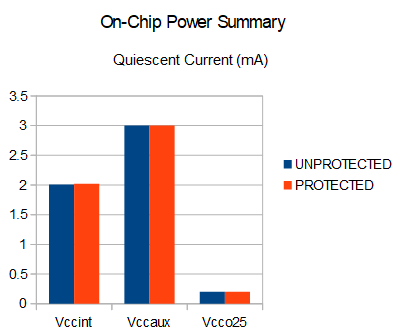
\includegraphics[width=0.5\textwidth]
	{pics/quiescent_current.png}
	\caption{quiescentcurrent}
	\label{quiescent_current}
\end{figure}

\begin{table}[H]
	\centering
	\caption{Power Supply Currents}
	\label{tab:addlabel}%
	\begin{tabular}{|c|c|c|c|c|}
		\hline
		\rowcolor[rgb]{ .906,  .902,  .902} \multicolumn{5}{|c|}{Unprotected} \bigstrut\\
		\hline
		\rowcolor[rgb]{ .906,  .902,  .902} \multicolumn{1}{|p{4.93em}|}{Supply Source} & \multicolumn{1}{p{4.93em}|}{Supply Voltage} & \multicolumn{1}{p{4.93em}|}{Total Current (mA)} & \multicolumn{1}{p{4.93em}|}{Dynamic Current (mA)} & \multicolumn{1}{p{4.93em}|}{Quiescent Current (mA)} \bigstrut\\
		\hline
		Vccint & 1.20  & 2.95  & 0.94  & 2.01 \bigstrut\\
		\hline
		Vccaux & 2.50  & 3.00  & 0.00  & 3.00 \bigstrut\\
		\hline
		Vcco25 & 2.50  & 0.20  & 0.00  & 0.20 \bigstrut\\
		\hline
		\rowcolor[rgb]{ .906,  .902,  .902} \multicolumn{5}{|c|}{Protected} \bigstrut\\
		\hline
		\rowcolor[rgb]{ .906,  .902,  .902} \multicolumn{1}{|p{4.93em}|}{Supply Source} & \multicolumn{1}{p{4.93em}|}{Supply Voltage} & \multicolumn{1}{p{4.93em}|}{Total Current (mA)} & \multicolumn{1}{p{4.93em}|}{Dynamic Current (mA)} & \multicolumn{1}{p{4.93em}|}{Quiescent Current (mA)} \bigstrut\\
		\hline
		Vccint & 1.20  & 3.16  & 1.14  & 2.02 \bigstrut\\
		\hline
		Vccaux & 2.50  & 3.00  & 0.00  & 3.00 \bigstrut\\
		\hline
		Vcco25 & 2.50  & 2.00  & 0.00  & 0.20 \bigstrut\\
		\hline
	\end{tabular}%
\end{table}%

Dari hasil diatas terlihat kebutuhan arus pada FPGA meningkat dari 2.95 menjadi 3.16 atau sekitar 6.64\% pada suplay Vccint di 1.2 Volt.

% Table generated by Excel2LaTeX from sheet 'Pengujian'
\begin{table}[htbp]
	\centering
	\caption{Gate yang digunakan setelah kompilasi ke netlist}
	\label{tab:gate}%
	\begin{tabular}{|c|c|}
		\hline
		\rowcolor[rgb]{ .906,  .902,  .902} Gate Synthesys & Gates \bigstrut\\
		\hline
		\rowcolor[rgb]{ .906,  .902,  .902} Unprotected & \cellcolor[rgb]{ 1,  1,  1} 5234 \bigstrut\\
		\hline
		\rowcolor[rgb]{ .906,  .902,  .902} Protected & \cellcolor[rgb]{ 1,  1,  1} 5324 \bigstrut\\
		\hline
	\end{tabular}%
\end{table}%

Kompilasi menggunakan library standard dari mosis didapatkan banyaknya gate yang digunakan sebelum rangkaian dilindungi adalah 5234 dan meningkat menjadi 5324 setelah rangkaian diberi pelindung. Peningkatan jumlah gate yang digunakan meningkat sekitar 1.69\%. Artinya bila dilakukan generate dari netlist ke layout peningkatan luas layoutnya tidak terlalu signifikan.

Selanjutnya desain disimulasikan dengan FPGA dan kontroler